% !TeX document-id = {0be8c18c-9430-4e9a-bdd9-12beadebfebc}
% !TeX TXS-program:bibliography = txs:///biber
\documentclass[11pt]{beamer}

\usepackage[brazilian]{babel}

\uselanguage{portuguese}
\languagepath{portuguese}
\deftranslation[to=portuguese]{Theorem}{Teorema}
\deftranslation[to=portuguese]{theorem}{teorema}
\deftranslation[to=portuguese]{Example}{Exemplo}
\deftranslation[to=portuguese]{example}{exemplo}
\deftranslation[to=portuguese]{Lemma}{Lema}
\deftranslation[to=portuguese]{lemma}{Lema}
\deftranslation[to=portuguese]{Corollary}{Corolário}
\deftranslation[to=portuguese]{corollary}{corolário}
%\deftranslation[to=portuguese]{and}{e}


\usepackage[utf8]{inputenc}
\usepackage[T1]{fontenc}
\usepackage{lmodern}
\usepackage{amsmath}
\usepackage{amssymb}
\usepackage{mathtools}
\usepackage{color}
\usepackage{pgfplots}
\usepackage{tikz}
\usepackage{subcaption}
%\usepackage{appendixnumberbeamer}

\newenvironment{transitionframe}{
	\setbeamercolor{background canvas}{bg=yellow}
	\begin{frame}}{
	\end{frame}
}
\usetheme{default}
\usefonttheme{structuresmallcapsserif}

%% I use a beige off white for my background
\definecolor{MyBackground}{RGB}{255,253,218}
\useinnertheme[shadow]{rounded}
\setbeamercolor{block title}{bg=MyBackground}
\setbeamercolor{block body}{bg=MyBackground}
\setbeamercolor{example title}{bg=MyBackground}
\setbeamercolor{example body}{bg=MyBackground}


\newcommand{\blue}[1]{\textcolor{blue}{#1}}
\newcommand{\red}[1]{\textcolor{red}{#1}}
\newcommand{\purple}[1]{\textcolor{purple}{#1}}
\newcommand{\gray}[1]{\textcolor{gray}{#1}}
\setbeamertemplate{navigation symbols}{}
%\setbeamertemplate{page number in head/foot}[appendixframenumber]

%\usepackage{graphics}
\usepackage{graphicx}

\definecolor{blue_emph}{RGB}{0,114,178}
\definecolor{red}{RGB}{213,94,0}
\definecolor{yellow}{RGB}{240,228,66}
\definecolor{green}{RGB}{0,158,115}
\definecolor{purple}{RGB}{204,121,167}
\definecolor{orange}{RGB}{230,159,0}
\definecolor{lightblue}{RGB}{86,180,233}

%\setbeamercolor{frametitle}{fg=blue}
%\setbeamercolor{title}{fg=blue}
\setbeamertemplate{footline}[frame number]
\setbeamertemplate{navigation symbols}{} 
\setbeamertemplate{itemize items}{-}
%\setbeamercolor{itemize item}{fg=blue}
%\setbeamercolor{itemize subitem}{fg=blue}
\setbeamertemplate{enumerate items}[default]
%\setbeamercolor{enumerate subitem}{fg=blue}
\setbeamercolor{button}{bg=MyBackground,fg=blue}
\usefonttheme{structuresmallcapsserif}

%\setbeamercolor{section in toc}{fg=blue}
%\setbeamercolor{subsection in toc}{fg=red}
\setbeamersize{text margin left=1em,text margin right=1em} 


\usepackage{appendixnumberbeamer}
\usepackage{pdfpages}
\usepackage[
backend=biber,
uniquename=false,
uniquelist=false,
style=authoryear,
natbib=true
]{biblatex}
\addbibresource{../bibliography.bib}

\newenvironment{wideitemize}{\itemize\addtolength{\itemsep}{10pt}}{\enditemize}
\newenvironment{wideenumerate}{\enumerate\addtolength{\itemsep}{10pt}}{\endenumerate}
\newenvironment{halfwideitemize}{\itemize\addtolength{\itemsep}{0.5em}}{\enditemize}
\newenvironment{halfwideenumerate}{\enumerate\addtolength{\itemsep}{0.5em}}{\endenumerate}


\author{Luis A. F. Alvarez}
\title{EAE1223: Econometria III}
\subtitle{Aula 10 - Heteroscedasticidade condicional}
%\logo{}
%\institute{}
\date{\today}
%\subject{}
%\setbeamercovered{transparent}

\def\signed #1{{\leavevmode\unskip\nobreak\hfil\penalty50\hskip2em
		\hbox{}\nobreak\hfil(#1)%
		\parfillskip=0pt \finalhyphendemerits=0 \endgraf}}

\newsavebox\mybox
\newenvironment{aquote}[1]
{\savebox\mybox{#1}\begin{quote}}
	{\signed{\usebox\mybox}\end{quote}}

\begin{document}

\begin{frame}[plain]
	\maketitle
\end{frame}

\begin{frame}{Log-retorno diário do Ibovespa}
\centering
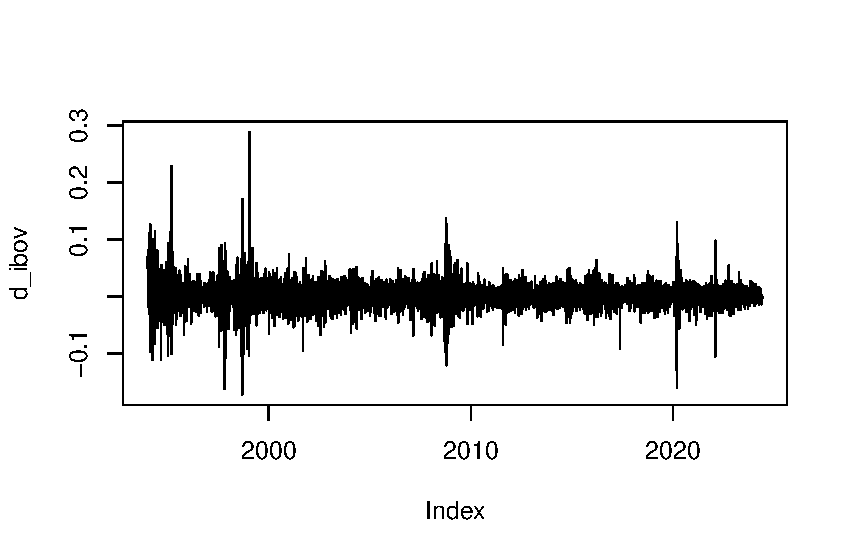
\includegraphics[scale=0.8]{plots/dibov.pdf}
\end{frame}

\begin{frame}{\textit{Clusters} de volatilidade}
\begin{halfwideitemize}
	\item Observe que os retornos diários exibem \textit{clusters} de volatilidade.
	\begin{halfwideitemize}
		\item Períodos de baixa variabilidade contrastam com períodos em que retorno varia mais.
	\end{halfwideitemize}
	\item O conceito probabilístico que captura este fenômeno é o de {\color{blue}heteroscedasticidade condicional}.
	\item Uma série de tempo $\{Y_t\}_{t \in \mathbb{Z}}$ exibe volatilidade condicional se a variância de $Y_t$, {\color{blue} condicional à informação $\mathcal{F}_{t-1}$ disponível até $t-1$}, varia no tempo.
	\item Isto é, definindo $\sigma_t^2 = \mathbb{V}[Y_t|\mathcal{F}_{t-1}]$, a série exibe heterocedasticidade condicional se  $\sigma^2_t$ varia no tempo.
	\begin{itemize}
		\item Se $\sigma^2_t$ é constante no tempo, temos homoscedasticidade condicional
	\end{itemize}
\end{halfwideitemize}
\end{frame}

\begin{frame}{Por que heteroscedasticidade condicional?}
\begin{halfwideitemize}
	\item Nas análises preditivas de nosso curso, focamos eminentemente em construir bom modelos para o valor esperado de $Y_{t+h}$ dada a informação disponível até $t$.
	\begin{halfwideitemize}
		\item Modelos univariados e multivariados para a {\color{blue}média condicional} de $Y_t$.
	\end{halfwideitemize}
		\item Por que focar na {\color{blue}variância condicional}?
	\begin{halfwideenumerate}

		\item Ganhos de eficiência: métodos de estimação derivados sob a hipótese de erros iid (o que exclui homoscedasticidade condicional) são {\color{blue}ineficientes} sob a presença de heteroscedasticidade condicional.
		\item Inferência: similarmente, métodos de inferência derivados sob a hipótese de erros iid são no geral {\color{blue}inválidos} sob a presença de intervalos de heteroscedasticidade condicional.
		\item  Por fim, nosso interesse pode residir em {\color{blue}estimar} a volatilidade fora da amostra, condicional à informação disponível até hoje.
		\begin{itemize}
			\item Importante na construção de carteiras de ativos e análises de risco.
		\end{itemize}
		\end{halfwideenumerate}
\end{halfwideitemize}
\end{frame}

\begin{frame}{Heteroscedasticidade condicional no ARMA(p,q)}
\begin{itemize}
	\item Considere um modelo ARMA(p,q) estacionário:
	$$\Phi(L)Y_t = \Theta(L)\epsilon_t \, .$$
	\item Se os ruídos brancos $\{\epsilon_{t}\}_t$ são \textbf{iid}, então, $\mathbb{V}[Y_{t+1}|\mathcal{F}_t] = \mathbb{V}[\epsilon_{t+1}|\mathcal{F}_t] = \mathbb{V}[\epsilon_{t+1}]  = \sigma^2_{\epsilon}$.
	\begin{itemize}
		\item Modelo exibe homoscedasticidade condicional.
	\end{itemize}
	\item Como incorporar heteroscedasticidade condicional?
		\item Para isso, vamos supor que:
		
		$$\epsilon_t = \sigma_t \nu_t  \, ,$$
		onde $\{\nu_t\}$ é iid  com  média zero e variância unitária e $\sigma_t = g(\mathcal{F}_{t-1})$ com $\mathbb{E}[\sigma^2_{t}] = \phi^2 < \infty$ para todo $t \in \mathbb{N}$.
\end{itemize}
\end{frame}

\begin{frame}{Propriedades }
\begin{itemize}
	\item Usando as propriedades de esperança condicional, é possível mostrar que o erro com a estrutura anterior exibe as seguintes propriedades:
	\begin{enumerate}
		\item $\mathbb{E}[\epsilon_t|\mathcal{F}_{t-1}] = 0$
		\item $\mathbb{V}[Y_t|\mathcal{F}_{t-1}]  = \mathbb{V}[\epsilon_t|\mathcal{F}_{t-1}] = \mathbb{E}[\epsilon_t^2|\mathcal{F}_{t-1}] = \sigma^2_t$.
		\item $\{\epsilon_t\}_t$ é de fato um ruído branco, com variância dada por $\mathbb{V}[\epsilon_t] = \phi^2 < \infty$. 
		\item $\operatorname{cov}(\epsilon_t^2, \epsilon_{t-s}^2) =\mathbb{E}[\sigma^2_t \sigma^2_{t-s} v_{t-s}^2] -  \phi^4$.
	\end{enumerate}
\end{itemize}
\end{frame}


\begin{frame}{Detectando heteroscedasticidade condicional}
\begin{itemize}
	\item Com base num modelo ARMA(p,q) estimado, como detectar a presença de heterocedasticidade condicional?
	\item Note que, do último item anterior, caso haja homoscedasticidade condicional, i.e. $\sigma^2_t=\sigma^2_{t-s} = \phi^2$, $\forall s \neq 0$, então $\operatorname{cov}(\epsilon_t^2, \epsilon_{t-s}^2)= 0$.
	\begin{itemize}
		\item Se há heteroscedasticidade condicional, então, no geral $\operatorname{cov}(\epsilon_t^2, \epsilon_{t-s}^2) \neq 0$.
	\end{itemize}
	\item Isso sugere testar a hipótese nula de homoscedasticidade condicional aplicando-se um {\color{blue}teste de Ljung-Box no quadrado dos resíduos} do modelo ARMA(p,q).
	\item Um teste alternativo segue da observação de que, sob homocedasticidade, $\mathbb{E}[\epsilon_t^2|\mathcal{F}_{t-1}]$ é constante e não depende de $\mathcal{F}_{t-1}$.
	\item Isso sugere usar os resíduos quadrados para ajustar um modelo linear:
	$$ \epsilon_t^2  = \psi_0 + \sum_{l=1}^k \psi_l \epsilon_{t-l}^2 + \xi_t$$
	e testar a nula  conjunta de que $\psi_1 = \psi_2 =\ldots = \psi_k=0$ usando um teste $F$.
\end{itemize}
\end{frame}

\begin{frame}{Modelo ARCH}
\begin{itemize}
	\item O modelo mais simples para heteroscedasticidade condicional é conhecido como {\color{blue}ARCH(m)}. Este modelo impõe que:
	
	$$\sigma^2_t = \omega_0 +\sum_{l=1}^m \omega_l \epsilon_{t-l}^2 \, ,$$
	com $\omega_j \geq 0$, $j=0,1\ldots, m$, e os parâmetros  $\omega_j$ restritos de tal forma que a variância incondicional seja finita.
	\item Neste modelo, volatilidade de $\epsilon_t$ depende do que ocorreu com o quadrado  de $\epsilon_t$ nos $t$ últimos períodos.
	
\end{itemize}
\end{frame}

\begin{frame}{Identificação da ordem do modelo ARCH}
	\begin{itemize}
		\item Note que, como $\sigma^2_t= \mathbb{E}[\epsilon^2_t|\mathcal{F}_{t-1}]$, um modelo ARCH(m) consiste efetivamente num modelo AR(m) para o erro quadrado.
		\item Isso sugere usar os resíduos quadrados do modelo ARMA estimado para detectar  a ordem $m$ do ARCH.
		\begin{itemize}
			\item Encontramos $m$ olhando para a ordem de truncagem da FACP dos resíduos quadrados.
		\end{itemize}
	\end{itemize}
\end{frame}

\begin{frame}{Estimação}
\begin{itemize}
	\item Dado que o modelo ARCH(m) é um modelo AR(m) para os erros quadrados do modelo ARMA(p,q), uma maneira simples de estimar os parâmetros da heteroscedasticidade condicional consiste em estimar um AR(m) usando os resíduos quadrados do ARMA(p,q) estimado como observações.
	\item No entanto, este método de estimação é no geral ineficiente, visto que não havíamos levado em conta a heteroscedasticidade na estimação do ARMA(p,q) preliminar.
	\item Um estimador mais eficiente consiste em estimar os parâmetros do ARMA(p,q) e do ARCH(m) {\color{blue}conjuntamente}, sob uma hipótese sobre os erros $\nu_t$.
	\item Se considerarmos o estimador de máxima verossimilhança, sob a hipótese auxiliar de $\nu_t \overset{iid}{\sim} N(0,1)$, temos o estimador de um modelo ARMA-ARCH com inovações Gaussianas.
	\begin{itemize}
		\item Esse estimador é eficiente se $\nu_t$ de fato for Gaussiano, e é consistente mesmo que o erro não seja Gaussiano (pseudo-máxima verossimilhança).
	\end{itemize}
\end{itemize}
\end{frame}

\begin{frame}{Caudas pesadas}
\begin{halfwideitemize}
	\item Embora estimador de máxima verossimilhança derivado sob hipótese de normalidade das inovações seja consistente mesmo que Gaussianidade seja violada, perda de eficiência pode ser grande.
	\item Além disso, para análises de risco, é importante modelar corretamente a distribuição do erro, pois o cálculo da probabilidade de eventos extremos, $\mathbb{P}[Y_{t+h} > c|\mathcal{F}_{t-1}]$, depende da distribuição de $\epsilon$.
	\item Nesses casos, a literatura considerou estimadores de MLE sob distribuições alternativas, que acomodam a existência de {\color{blue}caudas pesadas} nos retornos.  
	\begin{itemize}
		\item Um dos mais populares consiste em tomar $\nu_t \overset{iid}{\sim} t_k$, e estimar os graus de liberdade $k$ conjuntamente aos demais parâmetros.
		\begin{itemize}
			\item Quando $k\to \infty$, temos a normal. Para valores finitos, $t$-de Student apresenta caudas mais pesadas que a normal.
		\end{itemize}
	\end{itemize}
	\item Esses estimadores são eficientes se distribuição do erro estiver correta.
	\vspace{-1em}
	\begin{itemize}
		\item No entanto, e em contraste com o MLE Gaussiano, o estimador dos parâmetros é no geral inconsistente se errarmos a distribuição do erro (não há robustez a má-especificação).
	\end{itemize}
\end{halfwideitemize}
\end{frame}

\begin{frame}{Modelo GARCH}
\begin{halfwideitemize}
	\item A modelagem ARCH pode levar a escolhas de valores altos para $m$.
	\begin{itemize}
		\item Muitos parâmetros a se estimar, o que introduz o risco de sobreajuste. 
	\end{itemize}
	\item Nesses casos, modelos mais parcimoniosos podem ser encontrados se considerarmos um modelo GARCH(m,s):
$$\sigma^2_t  = \omega_0  +\sum_{l=1}^m \psi_l \epsilon^2_{t-l} + {\color{red}\sum_{l=1}^s \tau_l \sigma^2_{t-l}} \, .$$
onde os parâmetros são não negativos e de tal forma que a variância incondicional não exploda.
\item Ideia é incorporar dependência direta da heteroscedasticidade em seu valor pretérito, como forma de reduzir a necessidade de um $m$ alto.
\item Na literatura, geralmente se consideram ordens pequenas para $m$,$s$ (geralmente $1$ ou $2$)
\begin{itemize}
	\item Isso se deve à dificuldade computacional de se obter os estimadores de MLE para esse modelo.
	\item Não há método claro na literatura sobre como determinar $m$ ou $s$, para além do uso de critérios de informação no ranqueamento dos modelos.
\end{itemize}
\end{halfwideitemize}
\end{frame}

\begin{frame}{Validação}
\begin{halfwideitemize}
	\item Estimado um modelo (G)ARCH, obtemos estimativas da variância condicional, $\hat \sigma^2_t$, e do ruído branco, $\hat \epsilon_t$, na nossa amostra.
	\item Com base nessas estimativas, podemos calcular o resíduo estandardizado:
	$$\hat v_t = \frac{\hat \epsilon_t}{\hat \sigma_t}$$
	\item Com base nesse resíduo, podemos diagnosticar o modelo.
	\item Em particular, para um bom modelo, esperamos que $\hat \nu_t$ e $\hat \nu^2_t$ não exibam persistência, e que a distribuição de $\hat \nu_t$ esteja próxima daquela utilizada no MLE.
	\begin{itemize}
		\item Podemos verificar este último ponto usando gráficos quantil-quantil, comparando os quantis empíricos de $\hat \nu_t$ com os da distribuição de referência.
	\end{itemize}
\end{halfwideitemize}
\end{frame}

\begin{frame}{Outras alternativas}
Existe uma literatura enorme em Econometria Financeira, estendendo a modelagem GARCH.
		\begin{halfwideitemize}
			\item Modelos que acomodam assimetria no efeito dos choques $\epsilon_t$ sobre a volatilidade (EGARCH, TGARCH, etc.); que incorporam estocasticidade na evolução de $\sigma^2_t$ (modelos de volatilidade estocástica);  ou que incorporam o modelo da variância condicional diretamente no modelo para a média, capturando a relação risco-retorno nos ativos (M-GARCH).
			\item Também existe uma literatura que visa a construir procedimentos robustos na determinação de distribuições alternativas à normal, de modo a restaurar a propriedade de consistência do MLE Gaussiano sob má-especificação.
			\item Por fim, notamos que os modelos GARCH são extensíveis, também, à modelagem vetorial.
	\end{halfwideitemize}
\end{frame}
\end{document}

